\section{Semaine 18 (10/02-14/02) }


\e{Notions abordées :}
\begin{itemize}
	\item Équilibres acido-basiques.
	\item Titrages.
	\item Régime sinusoïdal forcé.
\end{itemize}

\subsection{Questions de cours}

\begin{enumerate}
	\item Définir la constante d'acidité.
	\item Quelles propriétés une réaction de titrage doit-elle vérifier ?
	\item Qu'est-ce que l'équivalence ? Montrer qu'à l'équivalence les réactifs ont été introduits dans les proportions stœchiométriques.
\end{enumerate}

\subsection{Exercice 1 : Le $pH$ sanguin}

L'activité métabolique et l'ingestion d'aliments peuvent introduire des espèces acido-basiques dans le sang. Or, la survie des cellules nécessite que le $pH$ varie très peu autour d'une valeur optimale. Ainsi le sang humain constitue un milieu tamponné : le $pH$ reste compris dans l’intervalle $7.36 - 7.44$ en temps normal.

\begin{enumerate}
	\item Tracer le diagramme de prédominance des espèces \ce{H2CO3}, \ce{HCO3-}, \ce{CO3^{2-}}, \ce{AH} et \ce{A-} sur un même axe de $pH$.
	\item Le sang est en partie tamponné par le couple \ce{H2CO3}/\ce{HCO3-} de concentration totale égale à $\SI{0.0280}{\mol\per\liter}$. Sachant que le $pH$ du sang vaut $\SI{7.40}{}$, calculer les concentrations en \ce{H2CO3} et \ce{HCO3-} avec trois chiffres significatifs.
	\item Dans certains cas, après des efforts physiques intenses, des crampes apparaissent. Il se forme alors dans les muscles de l'acide lactique \ce{AH} qui est transféré dans le sang.
	\begin{enumerate}
		\item Écrire l'équation de la réaction qui a lieu dans le sang et déterminer la valeur de sa constante d'équilibre.
		\item Dans le sang, après l'effort musculaire, dans un volume de $\SI{100}{mL}$ apparaît $\SI{3.0e-4}{\mol}$ d'acide lactique. Déterminer la composition du système à l'équilibre et en déduire la valeur du $pH$ local du sang. Conclure.
		\item Afin d'éviter cette variation du $pH$ sanguin l'hémoglobine et la respiration interviennent pour éliminer l'excès de dioxyde de carbone dissous, modélisé par \ce{H2CO3}. Expliquer qualitativement comment cela permet de maintenir constant la valeur du $pH$ sanguin. 
	\end{enumerate}
\end{enumerate}

\e{Données :}
\begin{itemize}
	\item L'acide l'actique est noté \ce{AH}, et sa base conjuguée \ce{A-}.
	\item $pKa(\ce{H2CO3}/\ce{HCO3-}) = \SI{6.1}{}$.
	\item $pKa(\ce{HCO3-}/\ce{CO3^{2-}}) = \SI{10.2}{}$.
	\item $pKa(\ce{AH}/\ce{A-}) = \SI{3.9}{}$.
\end{itemize}

\e{Réponses :}
\begin{enumerate}
	\item -
	\item $[\ce{H2CO3}] = \SI{1.34e-3}{\mol\per\liter}$ et $[\ce{HCO3-}] = \SI{2.67e-2}{\mol\per\liter}$
	\item -
	\begin{enumerate}
		\item \ce{AH} sur \ce{HCO3-}
		\item $pH = 6.8$
		\item -
	\end{enumerate}
\end{enumerate}

\subsection{Exercice 2 : Détermination d'une formule brute}

On veut déterminer par titrage la formule brute d'une amine \ce{C_nH_{2n+1}NH2}. Pour cela, on dissout une masse $m = \SI{0.146}{g}$ dans $\SI{100}{mL}$ d'eau et on dose la solution obtenue par une solution d'acide chlorhydrique de concentration molaire $c_A = \SI{0.25}{\mol\per\liter}$. On donne ci-contre la courbe de titrage $pH = f(V)$ à laquelle sont superposées en traits fins deux courbes représentant les pourcentages respectifs des espèces considérées.

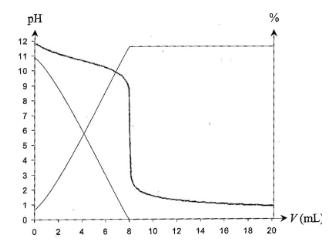
\includegraphics[width=\textwidth]{./Images/mpsi_s18_ex02.png}

\begin{enumerate}
	\item Attribuer les courbes de pourcentage aux espèces correspondantes et déterminer simplement le $pKa$ du couple.
	\item Écrire l'équation de la réaction. Calculer sa constante d'équilibre et justifier qu'elle peut servir de support de titrage.
	\item Justifier qualitativement l'allure de la courbe de $pH$.
	\item Proposer un indicateur coloré adapté au repérage de l'équivalence.
	\item Déterminer la formule de l'amine.
\end{enumerate}

\e{Données :}
\begin{enumerate}
	\item Masses molaires : $M_H = \SI{1.0}{\gram\per\mol}$, $M_C = \SI{12.0}{\gram\per\mol}$, $M_N = \SI{14.0}{\gram\per\mol}$.
	\item Zones de virage d'indicateurs colorés : phénolphtaléine $8.2$ à $10.2$, bleu de bromothymol $6.0$ à $7.6$, vert malachite $0.2$ à $1.8$.
\end{enumerate}

\e{Réponses :}
pKa = 10.7. n = 4.

\subsection{Exercice 3 : Titrage de l'acide acrylique}

On souhaite vérifier la concentration d'une solution d'acide acrylique noté \ce{AH} un peu ancienne (notée $S_0$). Il est écrit sur l'étiquette : $C_0 = \SI{6.25e-1}{\mol\per\liter}$. Pour cela, on décide de réaliser un titrage acido-basique.
On dispose d'une solution titrante de soude (\ce{Na+}, \ce{HO-}) de concentration $C_T = \SI{5.00e-2}{\mol\per\liter}$.

Avant dosage, la solution d'acide acrylique est diluée exactement vingt fois pour obtenir la solution $(S)$. Une prise d'essai $V_2 = \SI{20.0}{mL}$ de la solution $(S)$ est diluée par ajout d'un volume de $\SI{50}{mL}$ d'eau distillée, puis titrée par la solution  d'hydroxyde de sodium.

On note $V_0$ le volume total initial de la solution titrée, $V_T$ le volume de solution titrante ajouté et $V_E$ le volume versé à l’équivalence. Le titrage est suivi par pH-métrie. La courbe $pH = f(V_T)$  est donnée ci dessous.

On donne : $pKa(\ce{AH}/\ce{A-}) = 4.25$.

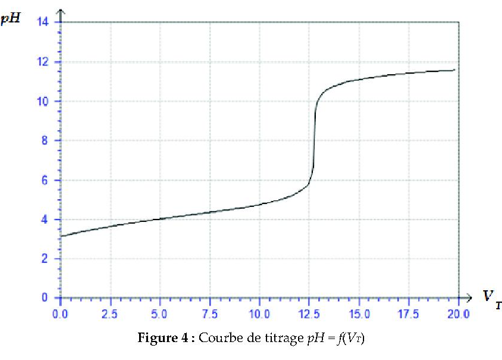
\includegraphics[width=\textwidth]{./Images/mpsi_s18_ex03.png}

\begin{enumerate}
	\item Écrire la réaction de dosage ainsi que la relation à l'équivalence.
	\item Calculer, en considérant que la concentration marquée sur l'étiquette est bonne, le $pH$ de la solution d'acide acrylique dans le bécher avant le début du titrage. Comparer à la valeur lue sur la courbe.
	\item Réciproquement, évaluer la vraie concentration en acide acrylique dans la solution $S$ à partir de la lecture du $pH$ à $V_T = 0$. Pourquoi n'utilise-t-on pas une seule mesure de $pH$, à la place d'un titrage, pour déterminer la concentration en acide acrylique dans la solution $S$ ?
	\item Déterminer la concentration en acide acrylique dans la solution $S$.
\end{enumerate}
